\section{Fazit}
\label{sec:Fazit}
Im Fazit sollen sowohl die technische Implementierung der Software als auch die Erfüllung der ursprünglichen Zielsetzung und der definierten Anforderungen analysiert und bewertet werden. Dabei werden die Projektphasen, die eingesetzten Technologien, die Qualität der Codebasis sowie die erreichten Funktionalitäten betrachtet. Des Weiteren werden etwaige Herausforderungen und Hindernisse während der Entwicklungsphase beleuchtet und mögliche Gründe für Abweichungen von der ursprünglichen Planung untersucht. Abschließend werden Empfehlungen zur Optimierung und Weiterentwicklung der Software formuliert.

\subsection{Zusammenfassung des Projektes}
\label{sec:Zusammenfassung}
Diese Arbeit widmete sich der Entwicklung eines Anwesenheitsplaners für das SMK mit dem Ziel, die Probleme der bestehenden Lösung mit Excel Dateien zu beheben. Dafür wurden die Phasen eines Softwareentwicklungsprojektes durchgeführt. Zuerst wurden die Probleme der bestehenden Lösung untersucht und mithilfe einer Anforderungsanalyse die funktionalen und nichtfunktionalen Soll-Anforderungen erhoben. Nach der Analyse wurde eine ausführliche Variantendiskussion durchgeführt die sowohl die Akquisition von Standartsoftware als auch eine Eingenentwicklung in betracht zog.

Es wurde sich für eine Eigenentwicklung entschieden, da keines der Verglichenen Softwaretool passen war. Für die Umsetzung wurden dann verschiedene Umsetzungsvarianten, wie WebApps und Desktopanwendungen verglichen. Am Ende wurde sich für die Entwicklung einer WebApp auf einer Monolitharchitektur entschieden. Als Framework für die Entwicklung wird Blazor Server eingesetzt.

Nach der Entscheidung für eine Umsetzungsvariante konnte auf Grundlage der Analyse der Entwurf der Software und des Systems erstellt werden. Für die Logik wurden Ablaufpläne und Klassendiagramme erstellt und die Systemarchitektur Skizziert. Das System soll am Ende aus einem Webserver, der die WebApp hostet und einer Datenbank besethen. Die Datenbank ist nur mit dem IIS Webserver verbunden und die Clients greifen nur auf den Webserver zu. Für die Erstellung der Datenbank wurde ein ERM auf Grundlage der in der Analysephase erstellten Referenztabelle.

In der letzten Phase wurden der Entwurf implementiert. Dazu wurde die Datenstruktur in der Datenbank angelegt und die WebApp in VisualStudio entwickelt. Es konnten erfolgreich alle funktionalen Anforderungen implementiert werden, jedoch musste dafür bei der Datenlogik und der Implementierung des MVVM Modells technische Schuld aufgebaut werden. Am ende konnte der Entwickelte Prototyp getestet werden, wobei der Abbau der technischen Schuld vor der Migration ins Live System gefordert wurde, da es Datenschutz- und Datensicherheitsrelevanz hat. Dementsprechend wird es eine zweite Entwicklungsphase geben in der die Fehler behoben werden sollen, damit das System in den Livebetrieb überführt werden kann.

\subsection{Vorstellung des Prototypen}
\label{sec:Prototyp}
Als Ergebnis wurde ein funktionsfähiger Prototyp erfolgreich entwickelt. Der Prototyp des Anwesenheitsplaners, ermöglicht es den Benutzern mit Single Sign-on auf die Weboberfläche zuzugreifen und dadurch die Anwesenheitsdaten einzusehen und zu setzten. Die Benutzeroberfläche, konnte sehr intuitiv gestaltet werden, was bei den Tests mit den Mitarbeitern sehr positiv aufgefasst wurde. Die Benutzeroberfläche des Prototypen siehe Abbildung \ref{abb:Prototyp} im Anhang.

\begin{figure}[htb]
    \centering
    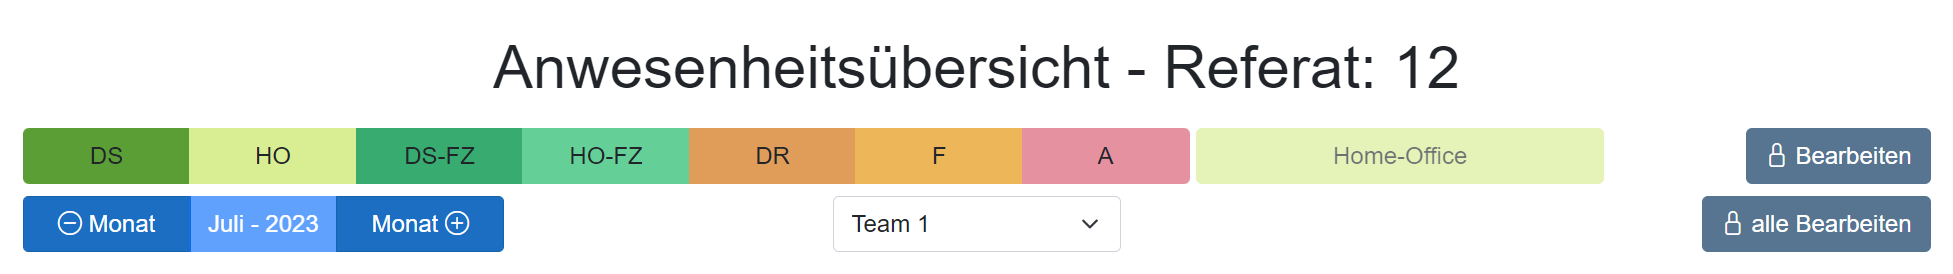
\includegraphics[width=1\textwidth,angle=0]{abb/Buttons_GUI.png}
    \caption[Beschreibung]{Schaltflächen}
    \label{abb:Buttons_GUI}
\end{figure}

Die Interaktion findet Hauptsächlich über die Schaltflächen über der Tabelle statt. Dort wird der einzutragende Anwesenheitsstatus ausgewählt, der dann durch das Klicken auf die Tabellenzelle für diesen Tag gesetzt wird. Die Schaltflächenübersicht siehe Abbildung \ref{abb:Buttons_GUI}. Über die Schaltflächen Bearbeiten und alle Bearbeiten kann zwischen den Lese- \bzw Schreibmodus gewechselt werden. Dabei ist die Schaltfläche alle Bearbeiten nur für Konten in der AD Gruppe AWPadmin mit einer Funktion hinterlegt.

Die Monatsansichten links in blau zeigen in der Mitte den aktuellen Monat und lassen sich mit den Schaltfläche links und rechts um je einen Monat verschieben. Als Letzte Schaltflächen kann der aktuell angemeldete Benutzer eine Teamzugehörigkeit auswählen, was die sortierung in der Tabelle ändert. Damit können referatsintern Substrukturen auf den Anwesenheitsplaner abgebildet werden.

Weitere Funktionen sind in Abbildung \ref{abb:Prototyp} im Anhang zu sehen. So sind \zB Feiertage und Wochenenden mit Gelb markiert und können keinen Anwesenheitsstatus bekommen. Der aktuelle Tag ist Rot markiert, im Fall der Abbildung der 18.07.2023.

\subsection{Soll-Ist-Vergleich}
\label{sec:Soll-Ist-Vergleich}
Der Soll-Ist-Vergleich zeigt, dass nahezu alle geplanten Funktionalitäten vollfunktional umgesetzt wurden. Die ursprünglich definierten funktionalen Anforderungen an das System wurden zufriedenstellend erfüllt. Das ist auf eine gute Analysephase zurückzuführen, dadurch die Referenztabelle bereits eine gute Vorlage für die zu entwickelnde Software vorhanden war. Allerdings haben die umfangreichen Tests auch einige Schwachstellen aufgezeigt. Insbesondere die Systemsicherheit und der Datenschutz müssen noch weiter verbessert werden, um den Prototypen für den Einsatz in produktiven Umgebungen fit zu machen. Insbesondere ein Datenschutzkonzept was aufbewahrungsfristen und den Umgang und Zugriff auf die Anwesenheitsdaten regelt muss von der Datenschutzbeauftrageten im SMK abgesegnet werden. Auch müssen im Bereich der Datensicherheit noch Nachbesserungen erfolgen. Ein kritikpunk ist \zB das Fehlende logging der WebApp. Es werden zwar Standartmaßgig vom Webserver und von der Datenbank Logs erzeugt, doch es ist wird ein spezifischeres Logging von Aktionen der Geschäftslogik gefordert. Auch sollten alle eingaben sowohl im Frontend als auch im Backend validiert werden um Fehlern vorzubeugen.

Abschließend ist zu sagen, dass der funktionale Soll-Zustand erreicht werden konnte, aber nur durch Abstriche in Codequalität und Sicherheitsfeatures.

\subsection{Bewertung der Umsetzung des Projektes}
\label{sec:Bewertung} %werden die Projektphasen,eingesetzten Technologien, die Qualität der Codebasis,Herausforderungen und Hindernisse während der Entwicklungsphase, Abweichungen von der ursprünglichen Planung
Die Umsetzung des Projektes verlief insgesamt positiv, da die solide Planung einen klaren Ablauf des Projektes definierte. Dabei gab es in der Planung und Analyse keine nennenswerten Schwierigkeiten. Das Änderte sich bei der Phase der Variantendiskussion, da keinerlei Vorwissen zu den Themen System- und Softwarearchitekturen vorhanden werden. Das erschwerte und verzögerte den Prozess der Auswahl einer Umsetzungsvariante, da das Wissen erst aufgebaut werden musste.

Die Auswahl der Technologien für die Umsetzung erwies sich im Nachhinein als sehr gelungen, da mit nur geringem Rechercheaufwand die benötigten Funktionalitäten umgesetzt werden konnten. Das lag vorallen Dingen an der Wahl des Csharp basierten Blazor Server Frameworks. Dadurch konnte ohne die Nutzung von Javascript eine vollfunktionale Weboberfläche erstellt werden. Nachteilig am einsatz des Frameworks war die geplante Anwendung des MVVM Musters für die Benutzerinteraktionen. Durch den Aufbau einer Razor Page muss das MVVM Muster anders als bei mit bekannten Frameworks implementiert werden, was dazu führte, dass das Muster nicht sauber Implementiert werden konnte. Das führe zu einer niedrigeren Qualität der Codebasis und sollte in der zweiten Entwicklungsphase erneut angegangen werden.

Die größten Schwierigkeiten lagen in der Umsetzung der Datenschutz- und Datensicherheitsrichtlinien. Hier gab es während Analyse, Entwurf und Implementierung immer wieder Rücksprachen mit den verantwortlichen im SMK. Doch richtige Maßnahmen für die geforderten Standarts des BSI zu finden und Umzusetzen gestaltete sich viel Zeitintensiver als erwartet. Deswegen musste von dem Plan ein Migrationsfertiges System zu entwickeln Abstand genommen werden und es wurde ein Prototyp entwickelt, der in einer zweiten Entwicklungsphase dann weiter angepasst werden soll.

\subsection{Ausblick}
\label{sec:Ausblick}



